\documentclass[11pt,a4paper]{article}
\usepackage[utf8]{inputenc}
\usepackage[T1]{fontenc}
\usepackage[english]{babel}
\usepackage{lmodern}
\usepackage{amsmath,amssymb}
\usepackage{bm}
\usepackage{booktabs,array}
\usepackage{graphicx}
\usepackage{tikz}
\usepackage[margin=2.5cm]{geometry}
\usepackage{hyperref}

\newcommand{\vm}{\bm{m}}
\newcommand{\vp}{\bm{p}}
\newcommand{\vs}{\bm{s}}
\newcommand{\vu}{\bm{u}}
\newcommand{\vphi}{\bm{\varphi}}
\newcommand{\Id}{\mathsf{I}}
\newcommand{\mK}{\mathsf{K}}
\newcommand{\ee}{\mathrm{e}}
\emergencystretch=3em

\title{Spin injection through a polarizer stack:\\
  angular test case on a thin free layer}
\author{}
\date{\today}

\begin{document}

\maketitle

\begin{abstract}
  This document comes with the validation case
  \texttt{validation/slonczewski\_angle} of the branch \texttt{slonczewski}
  of feeLLGood. It is the non-collinear companion of
  \texttt{validation/valet\_fert\_1d}: the magnetization of the polarizer
  makes an angle $\theta$ with the one of the free layer, the transverse
  spin current acts, and the mixing conductance of the circuit theory
  comes into play. The document explains the physics (spin-transfer
  torque, mixing conductance, absorption of the transverse spin current
  over the s--d length), the two models of the transverse spin current
  through the interface N/F2 offered by feeLLGood, the reference solution,
  and the expected results. In a limit, the damping-like torque has a
  closed form that shows why it only approximately follows the formula of
  Slonczewski.
\end{abstract}

\tableofcontents

\section{Purpose of the test}

On the branch \texttt{slonczewski}, the polarizer F1, the spacer N and the
interfaces F1/N and N/F2 are not meshed: they are replaced by a Robin
condition on the inlet surface of the free layer F2 (key
\texttt{slonczewski} of a surface region, \texttt{src/slonczewskiInterface.h},
\texttt{spinAcc::stackBoundaryCondition}). The collinear test
\texttt{valet\_fert\_1d} checks the longitudinal part of this condition.
This test checks its transverse part, the one that produces the
spin-transfer torque:
\begin{itemize}
  \item the conversion of the mixing conductance $G_{\uparrow\downarrow}$
    of the literature (in S/m$^2$) into the conductances of the spin
    diffusion problem, $G_r + iG_i = 2k\,G_{\uparrow\downarrow}$;
  \item the sign of the term in $\mathrm{Im}\,G_{\uparrow\downarrow}$;
  \item the two models of the transverse spin current through N/F2,
    \texttt{sink} (default) and \texttt{series};
  \item the coupling between the boundary condition and the
    non-collinear spin diffusion in F2 (precession, dephasing).
\end{itemize}
The reference is written independently of feeLLGood: the circuit theory
of Brataas, Bauer and Kelly for the interfaces, the equations of
feeLLGood solved exactly in F2.

\section{Physical background}

\subsection{Spin-transfer torque in a thin layer}

A current crossing a ferromagnet F1 becomes spin polarized along its
magnetization $\vp$. When it enters a second ferromagnet F2 of
magnetization $\vm\neq\pm\vp$, the component of its spin transverse to
$\vm$ is not an eigenstate there: it precesses around the exchange field
and dephases within a few ångströms to a nanometer. The angular momentum
it loses is transferred to the magnetization of F2: this is the
\emph{spin-transfer torque}. It has two components,
\begin{equation}
  \bm{\tau} = \tau_{\mathrm{DL}}\,\vm\times(\vm\times\vp)
            + \tau_{\mathrm{FL}}\,\vm\times\vp ,
\end{equation}
the \emph{damping-like} torque, which can compensate the damping and
switch the magnetization, and the \emph{field-like} torque, which acts like
a magnetic field along $\vp$. Slonczewski (1996, 2002) found for the
damping-like torque of a symmetric trilayer the angular dependence
\begin{equation}
  \tau_{\mathrm{DL}} \propto \varepsilon(\theta)\sin\theta,
  \qquad
  \varepsilon(\theta) = \frac{C}{(\Lambda^2+1)+(\Lambda^2-1)\cos\theta},
  \label{eq:slonczewski}
\end{equation}
$\cos\theta = \vm\cdot\vp$. For $\Lambda > 1$ the torque is larger near
the antiparallel configuration, for $\Lambda < 1$ near the parallel one.

In feeLLGood, the torque on the magnetization is proportional to
$\vm\times\vs$, where $\vs$ is the spin accumulation (in A/m), solution of
the spin diffusion problem. With $\vm = \hat z$ and $\vp$ in the plane
$(x,z)$, $\vm\times\vp$ is along $y$ and $\vm\times(\vm\times\vp)$ along
$-x$: the component $s_y$ gives the damping-like torque (since
$\vm\times\hat y = -\hat x$) and $s_x$ the field-like one.

\subsection{Mixing conductance}

In the circuit theory of Brataas, Bauer and Kelly, an interface between a
normal metal N and a ferromagnet F of magnetization $\vu$ is described by
its conductances. For the spin components along $\vu$, the majority
($\uparrow$) and minority ($\downarrow$) electrons conduct independently,
with conductances $G_\uparrow$, $G_\downarrow$: this is the collinear
model of Valet and Fert. For the components transverse to $\vu$, a new
conductance appears, the \emph{mixing conductance}
\begin{equation}
  G_{\uparrow\downarrow} = \frac{e^2}{h}\sum_{n}\Big[1 - \sum_m
    r_\uparrow^{nm}\big(r_\downarrow^{nm}\big)^*\Big]
  = G_r + iG_i \quad\text{(per unit area)},
\end{equation}
where $r_{\uparrow(\downarrow)}^{nm}$ are the reflection amplitudes, on the N
side, of the majority (minority) electrons from channel $m$ to channel
$n$. A transverse spin is a coherent superposition of $\uparrow$ and
$\downarrow$; after reflection, the two components have picked up
different amplitudes and phases. Only the overlap $r_\uparrow
r_\downarrow^*$ survives as transverse spin in N; the rest has been
absorbed by F:
\begin{itemize}
  \item $\mathrm{Re}\,G_{\uparrow\downarrow}$ measures the transverse
    spin absorbed: it produces the damping-like torque;
  \item $\mathrm{Im}\,G_{\uparrow\downarrow}$ measures the rotation of the
    reflected transverse spin around $\vu$: it produces a field-like
    torque.
\end{itemize}
For metallic interfaces, $\mathrm{Im}\,G_{\uparrow\downarrow}$ is usually
a few percent of $\mathrm{Re}\,G_{\uparrow\downarrow}$; here it is
deliberately large so that its sign matters.

\subsection{The interface law}

We use the variables of Valet--Fert: $j$ is the charge current density
along $+z$, $\vphi = \bm{\mu}_s/e$ the spin accumulation in volts
($\mu_s = (\mu_+-\mu_-)/2$ along the magnetization, $+$ = majority), and
$\bm{j}_s$ the spin current expressed as a charge current. The spin
current from the left (L) to the right (R) of an interface of
magnetization $\vu$ is
\begin{equation}
  \boxed{\;\bm{j}_s = \gamma\,j\,\vu + \mK(\vu)\,\Delta\vphi,
  \qquad
  \mK(\vu) = \frac{\vu\vu^{\mathsf{T}}}{AR^*}
    + 2G_r\left(\Id-\vu\vu^{\mathsf{T}}\right)
    + 2G_i\,[\,\cdot\times\vu\,]\;}
  \label{eq:interface}
\end{equation}
with $\Delta\vphi = \vphi_R-\vphi_L$ and $[\,\cdot\times\vu\,]$ the matrix
$\bm{w}\mapsto\bm{w}\times\vu$. Along $\vu$, it is the law of Valet--Fert,
$j_s = \gamma j + \Delta\varphi/AR^*$, with the interface resistance
$AR^*$ and asymmetry $\gamma$. Across $\vu$, it is the equation of Brataas
et al.\ for the transverse spin current from N into F,
$2G_r\,\vm\times(\bm{V}_S\times\vm) + 2G_i\,\bm{V}_S\times\vm$, with
$\bm{V}_S = -\vphi$ ($\mu = -eV$).

\paragraph{The factor 2.} For a non-magnetic interface ($\gamma = 0$,
$G_\uparrow = G_\downarrow = G_{\uparrow\downarrow} = G$ real), nothing
distinguishes the spin directions: the conductance must be isotropic. The
longitudinal one is $1/AR^* = G_\uparrow+G_\downarrow = 2G$, so the
transverse one must be $2G_{\uparrow\downarrow}$. This is the origin of
the factor 2 in \eqref{eq:interface}, and of the conversion
$G_r + iG_i = 2k\,G_{\uparrow\downarrow}$ of feeLLGood
(section~\ref{sec:feellgood}).

\paragraph{The sign of $\mathrm{Im}\,G_{\uparrow\downarrow}$.} It follows
from a single channel. A spin along $x$, $(|{\uparrow}\rangle +
|{\downarrow}\rangle)/\sqrt2$, is reflected into $(r_\uparrow|{\uparrow}\rangle
+ r_\downarrow|{\downarrow}\rangle)/\sqrt2$, whose transverse polarization is
$r_\uparrow^*r_\downarrow$ (as $\langle\sigma_x\rangle + i\langle\sigma_y
\rangle$). The transverse polarization absorbed is $1 - r_\uparrow^*
r_\downarrow = \overline{G_{\uparrow\downarrow}}$ (per channel, in units of
$e^2/h$): its imaginary part is $-G_i$, which fixes the sign of the last
term of \eqref{eq:interface}. The test checks that the opposite sign fails.

\subsection{Spin diffusion in the free layer}

In F2, feeLLGood solves
\begin{equation}
  \nabla\cdot Q = -\frac{\vs}{\tau_{sf}} - \frac{\vs\times\vm}{\tau_{sd}},
  \qquad
  Q_{i\alpha} = -P\,\frac{\mu_B}{e}\,j_i\,m_\alpha
  - D_0\left[\partial_i s_\alpha - P^2 m_\alpha(\vm\cdot\partial_i\vs)\right],
  \label{eq:zlf}
\end{equation}
with $D_0 = 2\sigma/(e^2N_0)$, $1/\tau_{sf} = D_0(1-P^2)/l_{sf}^2$ and
$1/\tau_{sd} = D_0/l_{sd}^2$; Latin indices denote space, Greek indices
the spin. In one dimension, with $\vm = \hat z$ uniform, the longitudinal
and transverse components decouple:
\begin{itemize}
  \item $s_z$: diffusion $D_0(1-P^2)$, relaxation over $l_{sf}$, as in
    Valet--Fert;
  \item $\psi = s_x + i s_y$: diffusion $D_0$ (not reduced), and
    $\vs\times\vm$ becomes $-i\psi$, so that
    \begin{equation}
      \psi'' = \kappa^2\,\psi,
      \qquad
      \kappa^2 = \frac{1-P^2}{l_{sf}^2} - \frac{i}{l_{sd}^2} .
    \end{equation}
\end{itemize}
With the parameters of the test, $\kappa = (0.718 - 0.697\,i)$\,nm$^{-1}$:
the transverse accumulation decays over $1/\mathrm{Re}\,\kappa = 1.39$\,nm
while rotating (wavelength $2\pi/|\mathrm{Im}\,\kappa| = 9.0$\,nm). The
spin current entering F2 polarized along $x$ precesses into $y$: this is
why $s_y$, hence the damping-like torque, appears in F2 even when
$G_i = 0$, and why $s_x$ changes sign across the layer
(figure~\ref{fig:profile}).

\paragraph{Torque and absorbed spin current.} Integrating the $x$
component of \eqref{eq:zlf} over the thickness $t_2$ ($(\vs\times\vm)_x =
s_y$):
\begin{equation}
  \frac{D_0}{l_{sd}^2}\int_0^{t_2} s_y\,dz
  = q_x(0) - q_x(t_2) - \frac{D_0(1-P^2)}{l_{sf}^2}\int_0^{t_2}s_x\,dz ,
\end{equation}
where $q_x = Q_{zx}$ is the flux of the $x$ component of the moment along
$z$. The integral of $s_y$, which measures the damping-like torque, is the
transverse spin current absorbed in the layer: the current entering at the
inlet, minus the one leaving at the outlet and the one relaxed by spin
flip. At $\theta = 90^\circ$ (\texttt{sink}), the three terms are
$17.15$, $-1.91$ and $0.14\times10^6$ (units of $\vs$ times m/s): the
inlet current dominates.

\subsection{Transverse spin current through N/F2: \texttt{sink} or \texttt{series}}

The circuit theory treats the ferromagnet as a node whose transverse spin
accumulation vanishes: the transverse spin current through N/F2 depends on
the accumulation of the spacer only. feeLLGood, however, also computes the
transverse accumulation of F2 near the interface. Two models are offered
(key \texttt{transverse} of \texttt{NF2}):
\begin{itemize}
  \item \texttt{sink} (default): the transverse spin current through N/F2
    depends on $\vphi_N$ only, as in the circuit theory. In
    \eqref{eq:interface}, $\vphi_F$ is replaced by its longitudinal part
    $\vm(\vm\cdot\vphi_F)$. $G_{\uparrow\downarrow}$ describes the whole
    absorption, and the diffusion in F2 only spreads the absorbed current
    over $l_{sd}$.
  \item \texttt{series}: it depends on $\vphi_N - \vphi_F$. The interface
    ($1/G_{r2}$) and the bulk of F2 ($1/g_\perp$, $g_\perp = D_0\kappa$)
    are then two absorption resistances in series, and
    $G_{\uparrow\downarrow}$ should be the part of the interface only
    (Petitjean, Luc and Waintal, 2012). With an \emph{ab initio}
    $G_{\uparrow\downarrow}$, which already contains the whole absorption,
    the absorption is counted twice.
\end{itemize}
Here $|2kG_{\uparrow\downarrow}| = 0.70\times10^6$\,m/s and $|g_\perp| =
2.32\times10^6$\,m/s: the bulk of F2 adds a resistance of about a third of
the one of the interface, and the damping-like torque is 15 to 17\,\%
smaller with \texttt{series}. The reference follows both models.

\section{The test case}

\subsection{Geometry and parameters}

\begin{figure}[h]
\centering
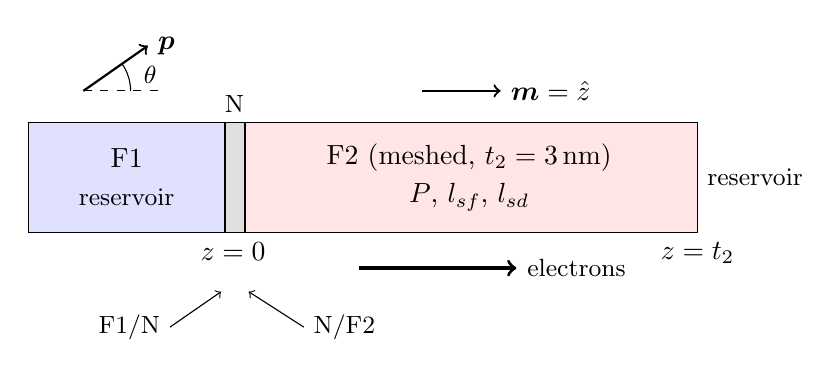
\begin{tikzpicture}[x=1cm,y=1cm]
  \fill[blue!12] (0,0) rectangle (2.5,1.4);
  \fill[gray!25] (2.5,0) rectangle (2.75,1.4);
  \fill[red!10] (2.75,0) rectangle (8.5,1.4);
  \draw (0,0) rectangle (8.5,1.4);
  \draw[thick] (2.5,0) -- (2.5,1.4);
  \draw[thick] (2.75,0) -- (2.75,1.4);
  \node at (1.25,0.95) {F1};
  \node at (1.25,0.45) {\small reservoir};
  \node at (5.6,0.95) {F2 (meshed, $t_2 = 3$\,nm)};
  \node at (5.6,0.45) {$P$, $l_{sf}$, $l_{sd}$};
  \draw[dashed] (0.7,1.8) -- ++(0:1.0);
  \draw[->,thick] (0.7,1.8) -- ++(35:1.0) node[right] {$\vp$};
  \draw (1.3,1.8) arc (0:35:0.6);
  \node at (1.55,2.0) {\small $\theta$};
  \draw[->,thick] (5.0,1.8) -- ++(0:1.0) node[right] {$\vm = \hat z$};
  \node[below] at (2.6,0) {$z=0$};
  \node[below] at (8.5,0) {$z=t_2$};
  \node[above] at (2.62,1.4) {\small N};
  \draw[<-] (2.45,-0.75) -- (1.8,-1.2) node[left] {\small F1/N};
  \draw[<-] (2.8,-0.75) -- (3.5,-1.2) node[right] {\small N/F2};
  \node[right] at (8.5,0.7) {\small reservoir};
  \draw[->,very thick] (4.2,-0.45) -- (6.2,-0.45) node[right] {\small electrons};
\end{tikzpicture}
\caption{The stack. Only F2 is meshed. The current flows along $z$, the
  magnetization of F1 is $\vp = (\sin\theta, 0, \cos\theta)$.}
\label{fig:stack}
\end{figure}

The stack is F1 (ideal reservoir, $\vphi = 0$) / F1/N / spacer N of zero
thickness / N/F2 / F2 / reservoir ($\vs = 0$), figure~\ref{fig:stack}. F2
is a layer of $2\times2$\,nm$^2$ and thickness $t_2 = 3$\,nm
(\texttt{thin\_layer.geo}, mesh size $h = 0.2$\,nm, 1\,695 nodes, P1
tetrahedra), which resolves $l_{sd} = 1$\,nm. Its side faces let through
neither charge nor spin: the problem is one-dimensional. The magnetization
of F2 is $\vm = \hat z$, the one of F1 is $\vp = (\sin\theta, 0,
\cos\theta)$, $\theta = 0, 30, \dots, 180^\circ$.

\begin{center}
\renewcommand{\arraystretch}{1.2}
\begin{tabular}{llll}
  \toprule
  Element & Parameter & Value & feeLLGood key \\
  \midrule
  F2 & $\sigma$ & $4\times10^6$\,S/m & \texttt{sigma} \\
    & $P$ & 0.5 & \texttt{P} \\
    & $l_{sf}$, $l_{sd}$ & 5\,nm, 1\,nm & \texttt{l\_sf}, \texttt{l\_sd} \\
    & $N_0$ & $1.344\times10^{47}$\,J$^{-1}$m$^{-3}$ & \texttt{dens\_state} \\
  F1/N & $AR^*$, $\gamma$ & $0.5\times10^{-15}\,\Omega\,$m$^2$, 0.75
    & \texttt{F1N.AR}, \texttt{F1N.gamma} \\
    & $G_{\uparrow\downarrow}$ & $(0.55 + 0.15\,i)\times10^{15}$\,S/m$^2$
    & \texttt{F1N.Gr}, \texttt{F1N.Gi} \\
  N/F2 & $AR^*$, $\gamma$ & $0.5\times10^{-15}\,\Omega\,$m$^2$, 0.75
    & \texttt{NF2.AR}, \texttt{NF2.gamma} \\
    & $G_{\uparrow\downarrow}$ & $(0.55 + 0.25\,i)\times10^{15}$\,S/m$^2$
    & \texttt{NF2.Gr}, \texttt{NF2.Gi} \\
    & model & \texttt{sink} or \texttt{series} & \texttt{NF2.transverse} \\
  Current & $j_n$ & $10^{12}$\,A/m$^2$ & \texttt{jn} (inlet) \\
  \bottomrule
\end{tabular}
\end{center}
F1 is an ideal reservoir: its bulk is not given (no key \texttt{F1}),
there is no renormalization. As in \texttt{valet\_fert\_1d}, $j_n > 0$ on
the inlet (outward normal $-z$) means that the electrons flow from F1 to
F2, and $j = -j_n$.

\section{Reference solution}

\subsection{The linear system}

In F2, the solution of \eqref{eq:zlf} with $\vs(t_2) = 0$ is a combination
of the three eigenmodes of $\left[D_0(\Id - P^2\vm\vm^{\mathsf{T}})\right]^{-1}
\left[D_0(1-P^2)/l_{sf}^2\,\Id + D_0/l_{sd}^2\,[\,\cdot\times\vm\,]\right]$,
of eigenvalues $1/l_{sf}^2$ and $\kappa^2$, $\bar\kappa^2$:
\begin{equation}
  \vs(z) = \sum_{n=1}^{3} c_n\,\bm{v}_n\,\sinh\left(\kappa_n(t_2-z)\right).
\end{equation}
The three coefficients $c_n$ and the accumulation $\vphi_N$ of the spacer
(six unknowns) are given by:
\begin{enumerate}
  \item the conservation of spin in the spacer, $\bm{j}_{s1} = \bm{j}_{s2}$,
    with \eqref{eq:interface} for F1/N ($\vu = \vp$, $\vphi_L = 0$,
    $\vphi_R = \vphi_N$) and N/F2 ($\vu = \vm$, $\vphi_L = \vphi_N$,
    $\vphi_R = \vphi_F$, replaced by $\vm(\vm\cdot\vphi_F)$ for
    \texttt{sink});
  \item the continuity of the moment flux at the inlet of F2:
    $Q_z(0) = -(\mu_B/e)\,\bm{j}_{s2}$,
\end{enumerate}
with $\vs = \mu_BN_0\,e\,\vphi/2$ (\texttt{validation/valet\_fert\_1d}).
This is the function \texttt{reference} of the script.

\subsection{Circuit reading: a closed form of the damping-like torque}
\label{sec:closed}

The system has a closed form for the model \texttt{sink} with
$G_{i1} = G_{i2} = 0$. Then:
\begin{itemize}
  \item the transverse current through N/F2 is $-2G_{r2}\,\vphi_{N\perp}$;
  \item along $\vm$, the interface N/F2 and the bulk of F2 are two elements
    in series, as in \texttt{valet\_fert\_1d}: polarization
    $P_2' = (\gamma_2AR_2^* + PR_2)/(AR_2^* + R_2)$ and conductance
    $G_\parallel' = 1/(AR_2^*+R_2)$, with the spin resistance of F2
    $R_2 = \rho^*l_{sf}\tanh(t_2/l_{sf})$, $\rho^* = 1/(\sigma(1-P^2))$;
  \item $\vphi_N$ stays in the plane $(\vm, \vp)$; the conservation in the
    spacer is a $2\times2$ system on its components along $\vm$ and
    $\hat x$.
\end{itemize}
With $a = 1/AR_1^* - 2G_{r1}$, $A = 2G_{r1} + G_\parallel'$ and
$B = 2G_{r1} + 2G_{r2}$, its solution gives the transverse spin current
entering F2:
\begin{equation}
  \boxed{\;j_{s\perp} = 2G_{r2}\,j\,
  \frac{\left(\gamma_1A + aP_2'\cos\theta\right)\sin\theta}
       {A(B+a) + a(B-A)\cos^2\theta}\;}
  \label{eq:closed}
\end{equation}
It agrees with the reference to $4\times10^{-4}$ (the difference being the
finite-difference derivative used for the comparison).

\paragraph{At $\theta = 90^\circ$,} $B + a = 1/AR_1^* + 2G_{r2}$ and
\begin{equation}
  j_{s\perp} = \gamma_1\,j\,\frac{2G_{r2}}{1/AR_1^* + 2G_{r2}} :
\end{equation}
F1/N is a Norton source $\gamma_1j$ along $\vp = \hat x$ of internal
conductance $1/AR_1^*$, loaded by the mixing conductance $2G_{r2}$ of N/F2.
Here $2G_{r2} = 1.1\times10^{15}$ and $1/AR_1^* = 2\times10^{15}$\,S/m$^2$:
35\,\% of the polarized current $\gamma_1 j$ is absorbed by F2.

\paragraph{Slonczewski's form.} The torque \eqref{eq:closed} has a
numerator linear in $\cos\theta$ and a denominator in $\cos^2\theta$; the
form \eqref{eq:slonczewski} has a constant numerator and a denominator
linear in $\cos\theta$. They differ in general: the structure here (an
ideal reservoir on one side, a thin layer on the other) is far from the
symmetric trilayer of Slonczewski. A fit gives $\Lambda^2 \approx 0.53$
(\texttt{sink}) and 0.54 (\texttt{series}) with a deviation of 4 to 5\,\%:
the torque is larger near the parallel configuration.

\section{What feeLLGood solves}
\label{sec:feellgood}

The function \texttt{Slonczewski::makeStack} converts each interface into
the units of the spin diffusion problem, with $k = 2/(e^2N_0)$ and the
density of states $N_0$ of F2:
\begin{equation}
  G_\parallel = \frac{k}{AR^*},\qquad P = \gamma,\qquad
  G_r + iG_i = 2k\,G_{\uparrow\downarrow}\quad[\mathrm{m/s}] ,
\end{equation}
builds the $3\times3$ conductance matrices $\mathsf{G}_1(\vp)$ and
$\mathsf{G}_2(\vm_0)$ of both interfaces at each node of the inlet, from
the trace $\vm_0$ of the magnetization, and eliminates the spacer
(\texttt{effectiveBC}). The result is the Robin condition
\begin{equation}
  \bm{q} = \frac{\mu_B}{e}\,j_n\,\bm{P}_{\mathrm{eff}}(\vm_0)
    - \mathsf{G}_s(\vm_0)\,\vs,
  \qquad
  \mathsf{G}_s = \mathsf{G}_2\mathsf{A}^{-1}\mathsf{G}_1,\quad
  \bm{P}_{\mathrm{eff}} = P_1\,\mathsf{G}_2\mathsf{A}^{-1}\vp
    + P_2\,\mathsf{G}_1\mathsf{A}^{-1}\vm_0,
\end{equation}
$\mathsf{A} = \mathsf{G}_1 + \mathsf{G}_2$, $P_{1,2} = \gamma_{1,2}$ the
polarizations of the interfaces, $\bm{q}$ the moment flux entering F2.
For \texttt{sink}, $\mathsf{G}_s$ is replaced by
$\mathsf{G}_s\vm_0\vm_0^{\mathsf{T}}$: only the longitudinal part of $\vs$
acts back on the interface. The reference reaches the same solution by
another route (the spacer and the interfaces are kept, in the variables of
Valet--Fert), so that an error in the elimination, the conversion or the
sign would show.

\section{Expected results}

\subsection{Torques}

\begin{figure}[h]
\centering
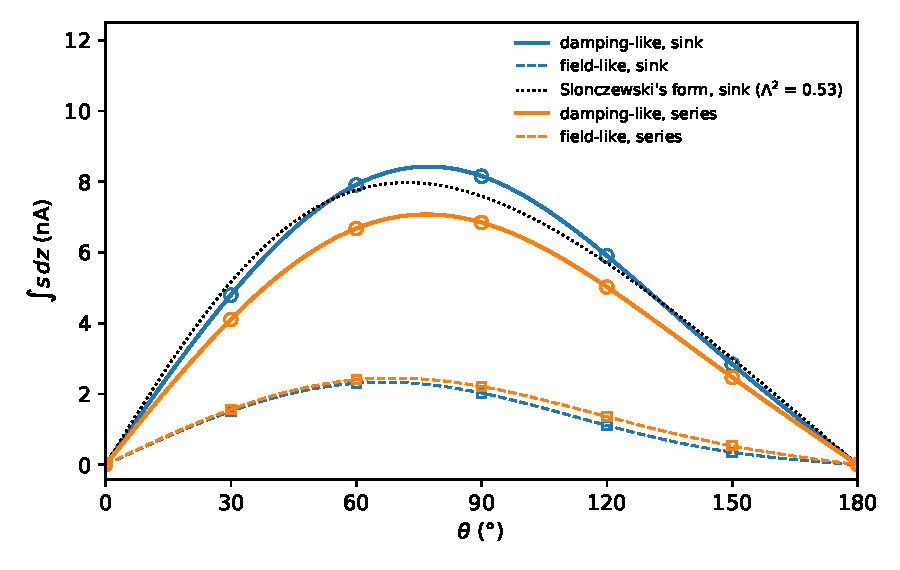
\includegraphics[width=0.85\textwidth]{slonczewski_angle_torque.pdf}
\caption{Damping-like ($\int s_y\,dz$, solid lines and circles) and
  field-like ($\int s_x\,dz$, dashed lines and squares) accumulations
  integrated over the thickness of F2: reference (lines) and feeLLGood
  (symbols), models \texttt{sink} and \texttt{series}. Dotted: form of
  Slonczewski fitted to the damping-like torque (\texttt{sink}).}
\label{fig:torque}
\end{figure}

Figure~\ref{fig:torque} and the tables below give the accumulations
integrated over the thickness (in A), which measure the torques. At 0 and
$180^\circ$, the transverse accumulation vanishes.

\begin{center}
\small
\renewcommand{\arraystretch}{1.15}
\begin{tabular}{rccc}
  \toprule
  \multicolumn{4}{c}{\texttt{transverse: sink} (default)} \\
  $\theta$ & damping-like $\int s_y\,dz$ & field-like $\int s_x\,dz$ & max error \\
  & feeLLGood / ref ($10^{-9}$\,A) & feeLLGood / ref ($10^{-9}$\,A) & on $\vs$ \\
  \midrule
  30  & 4.7941 / 4.7930 & 1.5079 / 1.5266 & $4.6\times10^{-3}$ \\
  60  & 7.9075 / 7.9065 & 2.2985 / 2.3291 & $1.1\times10^{-2}$ \\
  90  & 8.1529 / 8.1531 & 2.0235 / 2.0547 & $5.2\times10^{-3}$ \\
  120 & 5.9018 / 5.9031 & 1.1078 / 1.1300 & $2.3\times10^{-3}$ \\
  150 & 2.8398 / 2.8410 & 0.35261 / 0.36310 & $1.0\times10^{-3}$ \\
  \midrule
  \multicolumn{4}{c}{\texttt{transverse: series}} \\
  \midrule
  30  & 4.1054 / 4.1033 & 1.5626 / 1.5755 & $4.1\times10^{-3}$ \\
  60  & 6.6736 / 6.6702 & 2.4030 / 2.4238 & $1.1\times10^{-2}$ \\
  90  & 6.8434 / 6.8403 & 2.2136 / 2.2346 & $4.6\times10^{-3}$ \\
  120 & 5.0217 / 5.0198 & 1.3620 / 1.3772 & $1.9\times10^{-3}$ \\
  150 & 2.4700 / 2.4694 & 0.53402 / 0.54143 & $7.6\times10^{-4}$ \\
  \bottomrule
\end{tabular}
\end{center}
The maximum error on $\vs$, relative to $\max|\vs|$, stays below
$1.2\times10^{-2}$. The damping-like accumulation is reproduced to a few
$10^{-4}$, the field-like one to 1 to 3\,\%: $s_x$ changes sign across the
layer (figure~\ref{fig:profile}), and its integral results from a
cancellation, which magnifies the relative error.

\subsection{Profiles}

\begin{figure}[h]
\centering
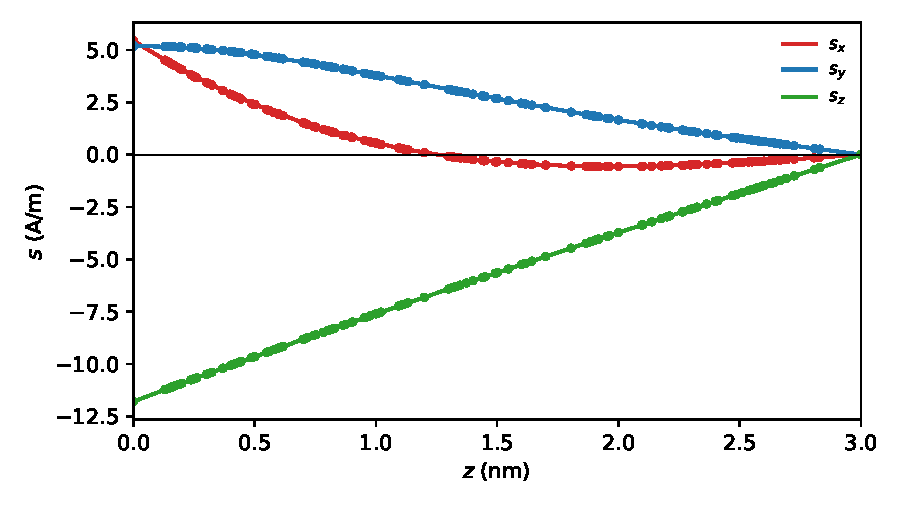
\includegraphics[width=0.8\textwidth]{slonczewski_angle_profile.pdf}
\caption{Components of $\vs$ across F2 at $\theta = 90^\circ$
  (\texttt{sink}): reference (lines) and feeLLGood at 200 randomly chosen
  nodes (circles).}
\label{fig:profile}
\end{figure}

Figure~\ref{fig:profile} shows the three components at $\theta =
90^\circ$. The transverse current enters polarized mainly along $x$:
$s_x$ is maximum at the inlet, then rotates into $y$ and changes sign at
about 1.2\,nm, as expected from $\kappa$. $s_y$ decreases almost linearly
to the outlet reservoir. The longitudinal accumulation $s_z$ is negative:
at $90^\circ$, the current enters F2 less polarized along $\vm$ than F2
carries it in its bulk.

\subsection{Convergence and sensitivity}

The error decreases as $h^2$ ($1.1\times10^{-2}$ at $h = 0.2$\,nm,
$2.7\times10^{-3}$ at $h = 0.1$\,nm, checked with \texttt{series} and
$\mathrm{Im}\,G_{\uparrow\downarrow} = 0$). The test fails (tolerance
2\,\%) if:
\begin{itemize}
  \item the conversion is $k\,G_{\uparrow\downarrow}$ instead of
    $2k\,G_{\uparrow\downarrow}$ (\texttt{series},
    $\mathrm{Im}\,G_{\uparrow\downarrow} = 0$): error 170\,\%;
  \item the sign of the term in $\mathrm{Im}\,G_{\uparrow\downarrow}$ of the
    reference is reversed (\texttt{IM\_SIGN = -1}, \texttt{series}): error
    13\,\%, the field-like accumulation differing by a factor 2 at
    $150^\circ$;
  \item the model of the reference is not the one of feeLLGood: the two
    models differ by 15 to 17\,\% on the damping-like torque.
\end{itemize}

\subsection{Usage}

\begin{verbatim}
cd validation/slonczewski_angle
./slonczewski_angle.py [path to feellgood]     # default: ../../src/feellgood
./plot_figures.py                              # figures of this document
\end{verbatim}
The mesh is built with \texttt{gmsh} if missing. The script runs
feeLLGood for each model and angle (14 runs, about 20\,s), prints for each
angle the integrals above and the maximum error, and the fit to the form
of Slonczewski:
\begin{verbatim}
damping-like torque (reference): Lambda^2 = 0.5315,
    deviation from the form of Slonczewski 5.2e-02
\end{verbatim}
The exit status is 0 if the error is below 2\,\% at every angle.

\section{Limitations of the test}

\begin{itemize}
  \item F1 is an ideal reservoir: the renormalization by the bulk of F1 is
    checked by \texttt{valet\_fert\_1d}.
  \item The magnetization of F2 is uniform and fixed: the coupling with
    LLG, the torque acting on a moving magnetization, is shown by the
    example \texttt{examples/}\allowbreak\texttt{pillar\_slonczewski\_}\allowbreak
    \texttt{current\_density\_ramp1ns}.
  \item All regions have the same density of states: see
    \texttt{validation/two\_regions\_1d}.
  \item The test does not tell which of \texttt{sink} and \texttt{series}
    is physically right: this depends on what the given
    $G_{\uparrow\downarrow}$ contains (whole absorption or interface
    only).
\end{itemize}

\section*{References}

\begin{itemize}
  \item J.\,C.~Slonczewski, J.~Magn.\ Magn.\ Mater.\ \textbf{159}, L1
    (1996); \textbf{247}, 324 (2002): spin-transfer torque, angular
    dependence with the parameter $\Lambda$.
  \item A.~Brataas, G.\,E.\,W.~Bauer, P.\,J.~Kelly, Phys.\ Rep.\
    \textbf{427}, 157 (2006): magnetoelectronic circuit theory, mixing
    conductance.
  \item T.~Valet, A.~Fert, Phys.\ Rev.\ B \textbf{48}, 7099 (1993).
  \item S.~Zhang, P.\,M.~Levy, A.~Fert, Phys.\ Rev.\ Lett.\ \textbf{88},
    236601 (2002): non-collinear spin diffusion.
  \item C.~Petitjean, D.~Luc, X.~Waintal, Phys.\ Rev.\ Lett.\
    \textbf{109}, 117204 (2012): transverse spin currents in
    drift-diffusion, consistent interface conditions.
  \item V.~Baltz, \emph{The Basics of Electron Transport in Spintronics},
    EDP Sciences (2023), §4.2--4.6.
  \item \texttt{validation/valet\_fert\_1d/valet\_fert\_1d.tex}: the
    collinear test, the Valet--Fert model and the conversion
    $\vs = \mu_BN_0e\vphi/2$.
  \item \texttt{dev-notes/spin\_injection\_boundary\_conditions.md}:
    derivation of the Robin condition and implementation.
  \item \texttt{dev-notes/slonczewski\_polarisation.tex} (in French): the
    same derivation, in detail.
\end{itemize}

\end{document}
